\section{Preprocessing Methodology}\label{sec:prep}

We lost only 292 of \nRawRows rows (0.19\%), all of them people whose cancer answer was unknown, and ended with 0 missing values in the model-ready file.

\subsection{A logged, reproducible pipeline}\label{sec:pipeline}

We built the cleaning as a pipeline in Python (pandas, SciPy~\cite{scipy}, scikit-learn~\cite{sklearn}, statsmodels~\cite{statsmodels}) rather than as notebook cells run by hand:
\begin{itemize}
  \item each step lives in a script -- \file{build_regional_data.py} for the three regional sources and \file{build_clean_dataset.py} for NHIS;
  \item each step records its effect (rows, columns, missing cells) in \file{data/clean/before_after_summary.csv} and explains itself in \file{data/clean/cleaning_report.txt};
  \item the whole project runs from one entry point, \texttt{python run\_all.py} (Table~\ref{tab:pipeline-steps}), with every random step seeded (42).
\end{itemize}
That made every decision below (Table~\ref{tab:problems}) easy to review and easy to undo, and it guarantees that the numbers in this report are the numbers the code produces.

\subsection{Problems found and treatments applied}\label{sec:problems}

Table~\ref{tab:problems} lists every data-quality problem we found, what we did about it, why, and its measured effect.

\begin{table}[htbp]
\centering\footnotesize
\caption{Data-quality problems, the treatment applied, the reason, and its measured effect.}\label{tab:problems}
\begin{tabularx}{\textwidth}{@{}>{\raggedright\arraybackslash}p{3.5cm} >{\raggedright\arraybackslash}X >{\raggedright\arraybackslash}p{3.7cm} >{\raggedright\arraybackslash}p{3.0cm}@{}}
\toprule
Problem found & What we did & Why & Effect \\
\midrule
Five yearly files; education renamed \texttt{EDUCP\_A} from 2021; doctorate coded 11 only in 2019--2020 & stacked the years, mapped both names to one column, mapped code 11 to ``Graduate'' & same codes every year, so one schema works & \nRawRows rows $\times$ 20 columns \\
Possible duplicate people & built \texttt{person\_id} = year + household number and checked for repeats & NHIS interviews one adult per household per year, so the key is unique by design; the check guards against a stacking error rather than finding real duplicates & 0 duplicates found \\
No ready-made target; \texttt{LUNGCAN\_A} only asked to people who had any cancer & 0 = no cancer or another cancer; 1 = lung cancer; refused / don't know $\rightarrow$ row removed & ``don't know'' is not ``no'', and we never impute a target & 292 rows removed; \nAdults kept, \nCases cases \\
Missing values hidden as numbers (7/8/9, 97/98/99) & recoded every column to readable labels; those codes $\rightarrow$ missing & otherwise a model would read 97 as a real value & 4,424 hidden codes in 4 key columns became missing \\
Inconsistent categories (e.g.\ smoking codes 1, 2, 5 all mean ``current'') & merged into one label per meaning (Current / Former / Never) & one category per real-world meaning & 3 clean smoking groups \\
Regional sources at a finer level (monitor, state) than NHIS (region) & aggregated to 4 regions $\times$ 5 years, then a left join on region + year & public NHIS files only identify the region & 20 region-years; \nAdults rows before and after; 0 unmatched \\
Outliers & IQR rule on the 6 numeric columns plus a plausibility check of every flagged value (\S\ref{sec:outliers}) & remove what is impossible, not what is rare & 0 removed \\
Remaining missing values (at most 2.84\%, Fig.~\ref{fig:missing}) & categories $\rightarrow$ explicit Unknown; yes/no $\rightarrow$ 0 plus an \texttt{\_unknown} flag; age $\rightarrow$ training median (54) plus a flag & keep every row; no detectable link between missingness and the target (Table~\ref{tab:missing}) & 0 missing cells in the model-ready file \\
Features that are exact or near-exact combinations of several other features (\texttt{comorbidity\_count} = sum of 5 flags; complete one-hot groups summing to 1; region dummies vs the regional columns) -- invisible to a pairwise correlation filter & Rule 4 of feature selection: variance inflation factor (VIF) on training rows; dropped \texttt{comorbidity\_count} (kept for the EDA), one reference category per one-hot group and the region dummies & a linear model cannot be fitted with perfect multicollinearity, and its coefficients are unstable with near-perfect multicollinearity & VIF: \nInfVIF of \nFeaturesBefore features infinite $\rightarrow$ maximum \maxVIFshort (none above 10); \nFeaturesBefore $\rightarrow$ \nFeatures features \\
Leakage risk & never used \texttt{CANEV\_A} (``ever had any cancer'') as a feature; split before fitting anything & every case has \texttt{CANEV\_A} = yes, so it would reveal the answer & no feature derived from the target \\
\bottomrule
\end{tabularx}
\end{table}

\subsection{Missing values}\label{sec:missing}

Before filling any gap (Fig.~\ref{fig:missing}) we checked whether missingness itself carries information about the target. For every column with at least 1\% missing, we cross-tabulated ``value missing'' against lung cancer with a $\chi^2$ test (all expected counts $\geq 14.5$, so the test is valid).

\begin{figure}[htbp]
\centering
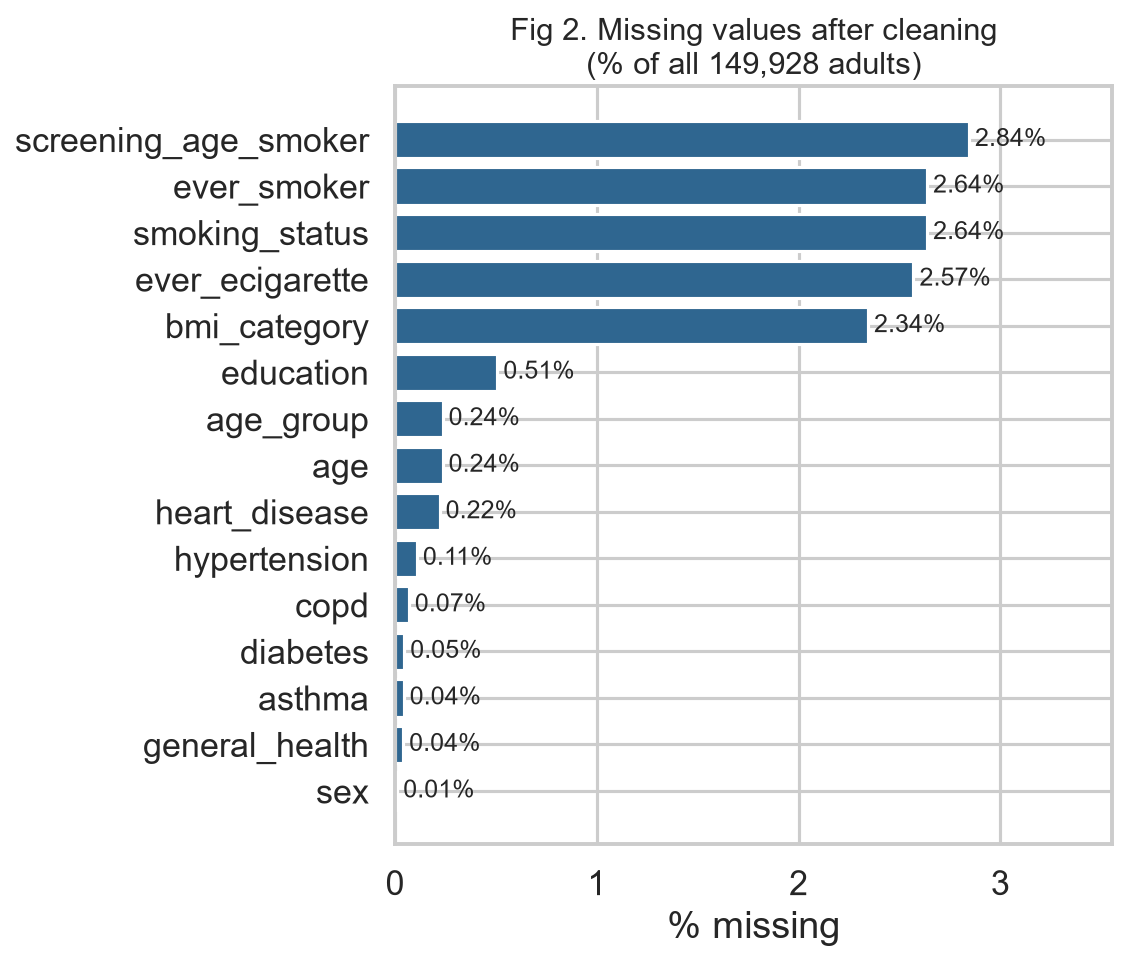
\includegraphics[width=0.55\textwidth]{fig02_missing_values}
\caption{Share of missing values per column after recoding the hidden ``unknown'' codes. The five smoking, e-cigarette and BMI columns are the only ones above 2.3\% (2.34--2.84\%); every other column is below 0.6\%.}\label{fig:missing}
\end{figure}

\begin{table}[htbp]
\centering\small
\caption{Is missingness related to lung cancer? $\chi^2$ tests of ``value missing (yes/no)'' $\times$ target.}\label{tab:missing}
\begin{tabular}{lrrrrrr}
\toprule
Column & \% missing & Rate if missing & Rate if present & $\chi^2$ & $p$ & Holm $p$ \\
\midrule
bmi\_category & 2.34 & 0.37\% & 0.41\% & 0.07 & 0.79 & 1.00 \\
ever\_ecigarette & 2.57 & 0.44\% & 0.41\% & 0.02 & 0.88 & 1.00 \\
smoking\_status / ever\_smoker & 2.64 & 0.46\% & 0.41\% & 0.09 & 0.77 & 1.00 \\
screening\_age\_smoker & 2.84 & 0.45\% & 0.41\% & 0.05 & 0.83 & 1.00 \\
\bottomrule
\end{tabular}

\end{table}

None of the differences is significant (all $p > 0.7$; Table~\ref{tab:missing}), so there is no detectable link between the gaps and lung cancer. We word this carefully: each missing group contains only about 14--18 expected cases, so the tests have little power, and they do not check whether missingness depends on other variables such as age or education. With at most 2.84\% missing per column, filling the gaps cannot move the main estimates much. We still keep an Unknown category or an \file{_unknown} flag wherever the gap is large enough to be informative, so a future model can learn from ``missing'' if it matters. Imputation values (the age median) are computed on training rows only (Section~\ref{sec:leakage}).

\subsection{Outliers}\label{sec:outliers}

The IQR rule flags values that are unusual, not values that are wrong (Fig.~\ref{fig:outliers}, Table~\ref{tab:outliers}). Removing the 7,451 adults with three or more chronic conditions would delete exactly the sick, older people among whom lung cancer is concentrated, and would bias every later estimate. Our rule was therefore to remove only impossible values; there were none.

\begin{figure}[htbp]
\centering
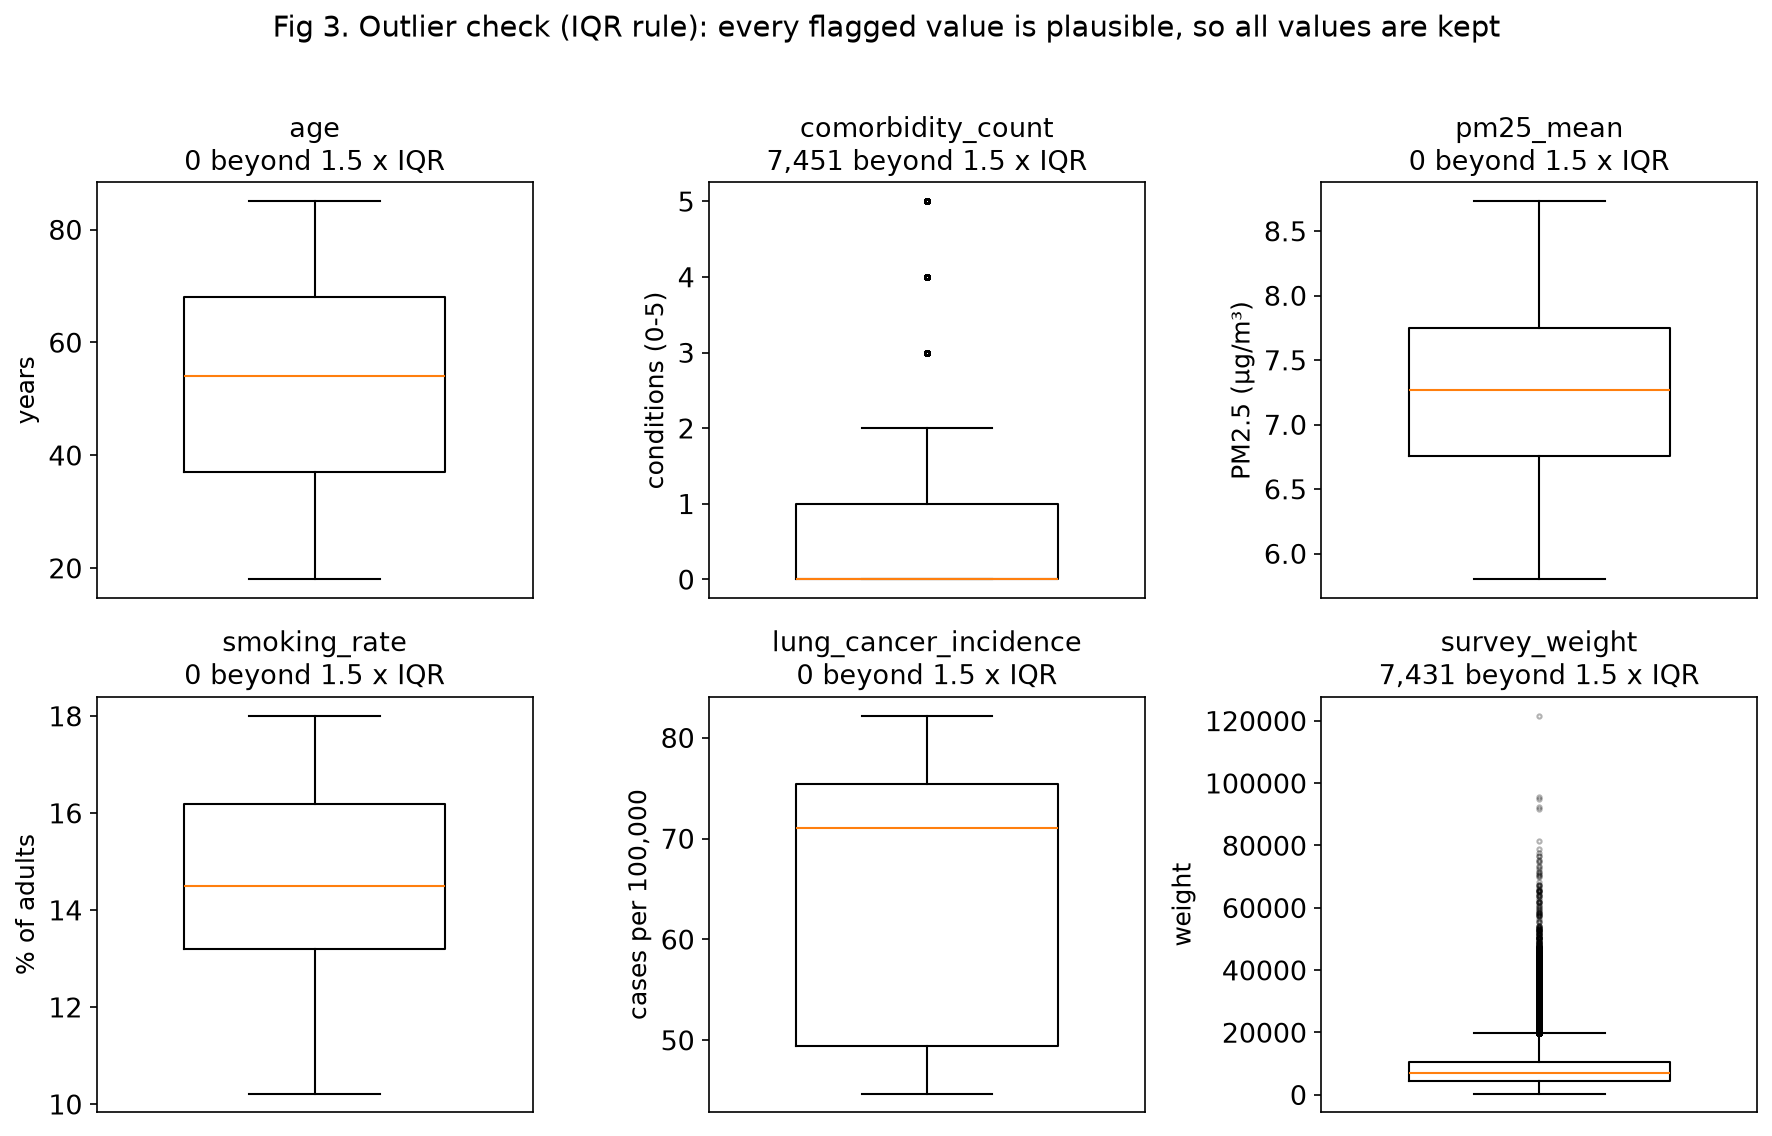
\includegraphics[width=0.85\textwidth]{fig03_outlier_boxplots}
\caption{Box plots of the six numeric columns with the number of values beyond $1.5 \times$ IQR. Every flagged value was checked for plausibility and kept.}\label{fig:outliers}
\end{figure}

\begin{table}[htbp]
\centering\small
\caption{Outlier check (IQR rule: below $Q_1 - 1.5 \times \mathrm{IQR}$ or above $Q_3 + 1.5 \times \mathrm{IQR}$) and the decision for each column.}\label{tab:outliers}
\begin{tabularx}{\textwidth}{l l r >{\raggedright\arraybackslash}X}
\toprule
Column & Bounds & Flagged & Decision and reason \\
\midrule
age & [$-$9.5, 114.5] & 0 (0\%) & keep -- every age 18-85 is a real adult; 85 means ``85 or older'' (NHIS top-code), not an error \\
comorbidity\_count & [$-$1.5, 2.5] & 7,451 (4.97\%) & keep -- a count from 0 to 5; high values are real people with several diseases \\
pm25\_mean & [5.3, 9.2] & 0 (0\%) & keep -- official EPA measurements; only 20 region-year values, none impossible \\
smoking\_rate & [8.7, 20.7] & 0 (0\%) & keep -- official CDC percentages between 0 and 100 \\
lung\_cancer\_incidence & [10.4, 114.4] & 0 (0\%) & keep -- official registry rates; differences between regions are real \\
survey\_weight & [$-$4883.8, 19849.6] & 7,431 (4.96\%) & keep -- NHIS design weight, used for population estimates only, not as a feature \\
\bottomrule
\end{tabularx}

\end{table}

\subsection{Integrating the regional sources}\label{sec:integration}

Each regional source needed its own cleaning before the three could be combined (\file{build_regional_data.py}; Table~\ref{tab:regional-cleaning}):

\begin{table}[htbp]
\centering\small
\caption{Cleaning and aggregation of the three regional sources.}\label{tab:regional-cleaning}
\begin{tabularx}{\textwidth}{@{}l >{\raggedright\arraybackslash}X >{\raggedright\arraybackslash}p{4.2cm}@{}}
\toprule
Source & Cleaning steps & Result \\
\midrule
EPA PM2.5 & kept the parameter ``PM2.5 -- Local Conditions'' and the official annual standard; kept ``No Events'' / ``Events Excluded'' rows (wildfire-type events removed); dropped values outside 0--100 \textmu g/m$^3$ and duplicate monitors; dropped 56 rows outside the 50 states + DC; averaged per state first (so states with many monitors do not dominate), then per region & 1,409--1,798 annual monitor values per year $\rightarrow$ 20 region-year means \\
BRFSS smoking & kept the ``current smoker = yes'' answer, years 2019--2023, values 0--100\%; dropped 21 territory / national rows; averaged per region & 1,644 rows $\rightarrow$ 251 state-years $\rightarrow$ 20 region-years \\
US Cancer Statistics & kept lung cancer, both sexes, all races, single years (multi-year rows dropped); suppressed counts treated as missing; region rate = sum of cases $\div$ sum of population $\times$ 100,000 & 23,796 rows $\rightarrow$ 255 state-years $\rightarrow$ 20 region-years \\
\bottomrule
\end{tabularx}
\end{table}

We mapped every state to its US Census region -- the same four regions NHIS uses -- and combined the three tables into one 20-row table (\file{data/clean/regional_context.csv}). No region-year was missing; the code would fill a missing year from the same region's nearest year and log it. The NHIS table was then left-joined on region + year with a many-to-one validation, and an assertion stops the pipeline if the join ever adds a row. Result: \nAdults rows before and after, 0 adults without a regional match.

Two aggregation choices are worth stating plainly because they are limitations: the registry rate is a crude rate (not age-adjusted), and states are averaged without population weights. Both are discussed in Section~\ref{sec:regional}.

\subsection{Effect of each step}\label{sec:effect}

Table~\ref{tab:before-after} follows the data through the pipeline. The column count changes for simple reasons: step 2 adds \file{person_id} ($20 \rightarrow 21$), step 3 adds the target (22), and step 4 replaces the raw NHIS columns with 19 readable ones (the helper columns \file{HHX}, \file{CANEV_A} and \file{LUNGCAN_A} are not carried forward). The missing cells fall sharply at step 4 because \file{LUNGCAN_A}, blank by design for everyone without cancer, is no longer carried; they rise again at step 5 only because the new columns inherit the gaps of the columns they are built from. The \nModelColumns columns of the model-ready file are the \nFeatures features plus \file{person_id}, \file{split}, \file{survey_weight} and the target.

\begin{table}[htbp]
\centering\footnotesize
\caption{Rows, columns and missing cells after each preprocessing step (\texttt{data/clean/before\_after\_summary.csv}).}\label{tab:before-after}
\begin{tabularx}{\textwidth}{>{\raggedright\arraybackslash}p{3.6cm} r r r >{\raggedright\arraybackslash}X}
\toprule
Step & Rows & Columns & Missing cells & What changed \\
\midrule
1. Load + stack 5 years & 150,220 & 20 & 131,400 & 5 yearly files stacked; 20 needed columns kept (LUNGCAN\_A is blank by design for people who never had cancer) \\
2. Remove duplicates & 150,220 & 21 & 131,400 & 0 duplicate person IDs removed \\
3. Build target & 149,928 & 22 & 131,217 & 292 rows with unknown answer removed \\
4. Recode codes $\rightarrow$ values & 149,928 & 19 & 13,235 & number codes turned into words; e.g. 4,424 ``unknown'' codes in 4 key columns $\rightarrow$ missing \\
5. New columns & 149,928 & 23 & 21,805 & added age\_group, ever\_smoker, screening\_age\_smoker, comorbidity\_count \\
5b. Join regional table & 149,928 & 26 & 21,805 & 3 columns added (pm25\_mean, smoking\_rate, lung\_cancer\_incidence); 0 rows added \\
5c. Outlier check & 149,928 & 26 & 21,805 & IQR check on 6 numeric columns; all values plausible $\rightarrow$ kept \\
6. Checks + save clean file & 149,928 & 26 & 21,805 & 0 duplicate IDs, ages 18-85, missing values listed \\
7. Encode + fill gaps (train only) & 149,928 & 71 & 0 & one-hot encoding, training-median filling, ``unknown'' flags $\rightarrow$ 0 missing \\
8. Feature selection & 149,928 & 42 & 0 & 29 redundant / near-constant / near-duplicate / linearly dependent features dropped; 38 kept (max VIF 7.5) \\
9. Scaling (train only) & 149,928 & 42 & 0 & 4 numeric columns standardised \\
\bottomrule
\end{tabularx}

\end{table}

\subsection{How we prevented data leakage}\label{sec:leakage}

We treated the test set like production data the model has never seen, following the leakage checklist of Kapoor and Narayanan~\cite{kapoor}:
\begin{itemize}
  \item The 80/20 split (stratified on the target, seed 42) happens before anything is learned from the data: \nTrain training rows and \nTest test rows, both with a \sampleRate\% case rate.
  \item The age median used for filling, the feature-selection rules and the VIF step, the scaler and the PCA are all computed on training rows only, then applied unchanged to the test rows.
  \item \file{CANEV_A} is never a candidate feature, \file{person_id} is an identifier only, and \file{survey_weight} is used for population estimates, never as a feature.
  \item A sanity check: after scaling, the training means are exactly 0 while the test means are slightly off ($-0.002$ for age, 0.006 for PM2.5, $-0.001$ for the regional smoking rate and 0.019 for registry incidence; Table~\ref{tab:scaler}). That is exactly what we expect if the scaler never saw the test rows, and \file{supplementary_analysis.py} turns it into an assertion: the saved scaler parameters must equal a refit on training rows only and must differ from a fit on all rows.
\end{itemize}

Descriptive statistics, the population profile and the hypothesis tests in Sections~\ref{sec:profile} and~\ref{sec:eda} use all adults, because they describe the population and fit nothing that a model reuses. Two design decisions were nevertheless informed by data on all rows, and we state them openly: merging the three smallest race groups for the $\chi^2$ test (a testing decision only; the model-ready file keeps all seven groups, with White as the reference), and the \file{screening_age_smoker} feature, which comes from the USPSTF rule~\cite{uspstf} and was only illustrated by Fig.~\ref{fig:agesmoking}. The one EDA step that ranks features (mutual information, \S\ref{sec:mi}) uses training rows only.
